% !TeX root = ../thuthesis-example.tex

\chapter{模型上下文协议}

模型上下文协议(Model Context Protocol, MCP)是一种标准化协议,旨在规范AI应用与各种数据源和工具之间的连接与交互方式。与传统的定制接口不同,MCP提供了一种通用的连接标准,使AI模型能够以一致的方式访问和操作外部资源。类似于USB-C为物理设备提供通用接口,MCP为AI应用提供了统一的数据交换和工具调用框架。在MCP出现之前,开发者需要为每个数据源或工具构建专用连接,这是一个耗时且限制功能的过程。如今,通过MCP,开发者可以轻松地为他们的AI应用添加外部资源连接,显著提升应用能力和实用性\cite{mcpspec2023}。

bolt.se的MCP模块就是这一协议的实际应用,它允许用户配置和管理外部MCP服务器,使大语言模型(LLM)能够通过标准化接口访问外部工具和数据。本章将详细介绍MCP的概念、意义、优势、对LLM驱动软件开发的重要性,以及bolt.se中MCP模块的实现方案。

\section{模型上下文协议的概念与意义}

\subsection{MCP在软件工程中的优势}
模型上下文协议为现代AI驱动的软件工程带来了显著的优势:

\begin{enumerate}
  \item \textbf{标准化工具集成}:MCP提供了统一的接口规范,使AI应用能够以一致的方式与各种外部工具和服务交互,大幅降低了集成复杂性。
  
  \item \textbf{解耦与可扩展性}:通过MCP,AI模型与工具实现完全解耦,使系统能够独立演化,新工具可以在不修改核心模型的情况下动态添加。
  
  \item \textbf{传输方式灵活性}:MCP支持多种传输协议(如stdio、HTTP SSE等),适应不同的部署环境和网络条件,提高了系统的适应性。
  
  \item \textbf{工具发现机制}:MCP内置的工具发现机制使AI模型能够动态了解可用工具的功能和参数,实现智能工具选择和调用。
  
  \item \textbf{安全性与边界控制}:MCP提供了清晰的权限边界,使AI模型只能通过受控接口访问外部资源,降低了安全风险。
\end{enumerate}

在bolt.se这样的现代开发平台中,MCP的这些优势使得开发者能够安全、灵活地扩展AI应用的能力边界,创造更加强大和实用的工具生态。

\subsection{MCP对LLM驱动软件开发的重要性}
在大型语言模型(LLM)驱动的软件开发范式中,MCP具有特殊且关键的意义:

\begin{enumerate}
  \item \textbf{克服知识截止限制}:通过MCP,LLM可以访问最新的外部数据和信息,突破训练数据截止日期的限制,保持信息的时效性。
  
  \item \textbf{功能边界拓展}:MCP允许LLM调用专业工具和API,执行其内在能力无法完成的任务,如数据分析、复杂计算、文件操作等,极大拓展了应用场景。
  
  \item \textbf{减少幻觉生成}:通过引导LLM从可靠的外部来源获取信息,而非依赖其参数化知识,MCP显著降低了幻觉(Hallucination)生成的可能性,提高了输出的准确性。
  
  \item \textbf{交互式问题解决}:MCP支持LLM与外部工具的多轮交互,使其能够分步骤解决复杂问题,验证中间结果并调整后续策略。
  
  \item \textbf{私有数据安全访问}:MCP提供了安全机制,使LLM能够在保护隐私的前提下访问用户的私有数据,平衡了功能性与安全性。
\end{enumerate}

在bolt.se中,MCP理念已经深度融入系统设计。通过将标准化的工具接口集成到开发流程中,bolt.se实现了LLM与外部工具和数据源的无缝协作,使开发者能够通过自然语言交互获得工具增强的智能辅助。这种结合不仅保留了LLM的灵活性和创造性,还增添了专业工具的精确性和功能扩展性,为软件开发带来了革命性的效率提升。

\section{MCP协议规范与工具类型}

MCP是一种开放的协议规范,为AI模型与外部上下文的交互提供了标准化接口。它定义了服务器与客户端之间的通信格式、传输方式以及工具定义和调用机制,使AI应用能够以一致的方式与各种外部资源交互\cite{mcpspec2023}。

\subsection{MCP协议规范简介}

MCP协议的核心组件包括:

\begin{enumerate}
  \item \textbf{传输层}:定义了客户端与服务器之间的通信机制,主要支持两种模式:
    \begin{itemize}
      \item \textit{stdio传输}:通过标准输入/输出流与本地进程通信,适合执行本地工具和命令。
      \item \textit{HTTP SSE传输}:通过HTTP Server-Sent Events与远程服务器通信,适合云服务和网络API。
    \end{itemize}
  
  \item \textbf{消息格式}:采用JSON格式的消息传递,包括以下类型:
    \begin{itemize}
      \item 握手消息:建立连接并交换版本信息
      \item 工具发现消息:获取可用工具及其模式定义
      \item 工具调用消息:请求执行特定工具及其参数
      \item 工具响应消息:返回工具执行结果
      \item 错误消息:报告执行过程中的问题
    \end{itemize}
  
  \item \textbf{工具模式}:使用JSON Schema定义工具的输入参数和输出格式,包括:
    \begin{itemize}
      \item 工具名称和描述:明确工具的功能和用途
      \item 参数定义:指定必需和可选参数,包括类型、格式和约束
      \item 返回值定义:指定输出的结构和类型
    \end{itemize}
\end{enumerate}

bolt.se支持的MCP服务器配置示例如下:

\begin{verbatim}
{
  "mcpServers": {
    "localFileSystem": {
      "type": "stdio",
      "command": "node",
      "args": ["./mcp-file-server.js"]
    },
    "weatherService": {
      "type": "sse",
      "url": "https://weather-mcp.example.com/connect"
    }
  }
}
\end{verbatim}

bolt.se的MCP模块能够解析这种配置,创建相应的MCP客户端,连接到指定的服务器,并获取可用的工具集。

\subsection{MCP支持的工具类型}

MCP协议支持多种类型的工具,满足不同的AI应用需求:

\begin{enumerate}
  \item \textbf{信息检索工具}:使LLM能够访问最新的外部数据,如网络搜索、文档查询、数据库访问等。
  
  \item \textbf{计算工具}:提供数学计算、统计分析、数据处理等能力,弥补LLM在精确计算方面的不足。
  
  \item \textbf{文件操作工具}:允许读取、写入、创建和删除文件,支持代码生成和文档处理。
  
  \item \textbf{API调用工具}:封装对第三方API的访问,如天气服务、地图服务、社交媒体API等。
  
  \item \textbf{系统交互工具}:提供与操作系统和本地环境的交互能力,如执行命令、管理进程等。
  
  \item \textbf{专业领域工具}:集成特定领域的专业工具,如代码分析、图形处理、自然语言处理等。
\end{enumerate}

在bolt.se中,这些工具通过MCP协议被动态发现和注册,使LLM能够根据具体任务需求选择和调用适当的工具,极大地扩展了系统的功能边界和应用场景。

MCP的开放性和可扩展性使开发者能够根据需求创建自定义工具,并通过标准接口与LLM集成,形成丰富的工具生态系统。bolt.se正是基于这一理念,提供了灵活的MCP配置和管理机制,支持用户扩展系统能力。

\section{bolt.se中的MCP实现}

bolt.se作为一个AI驱动的软件开发平台,将MCP深度融入其架构设计。系统通过结构化的MCP模块,使用户能够轻松配置、管理和应用外部MCP服务器,同时让大语言模型能够理解并调用这些服务提供的工具,实现功能扩展和技术集成。本节将详细介绍bolt.se中MCP的实现方案,从整体架构设计到具体功能实现。

\begin{figure}[htbp]
  \centering
  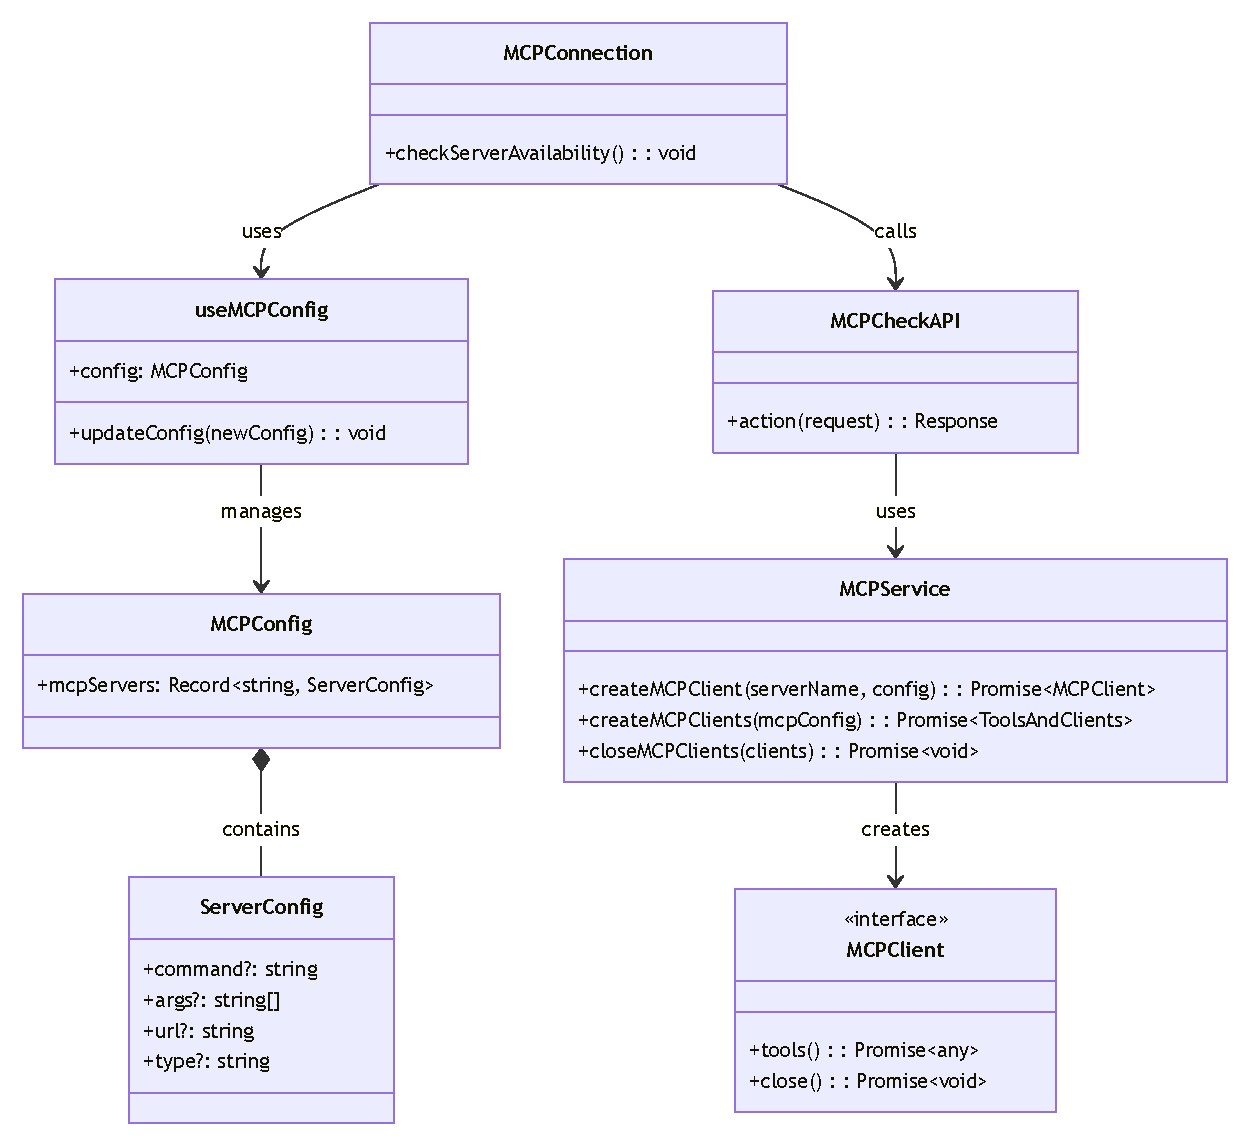
\includegraphics[width=\textwidth]{figures/mcp_class.pdf}
  \caption{MCP类图:展示了系统中MCP相关模块的类结构及其关系,包括配置管理、服务创建和连接检查}
  \label{fig:mcp_class}
\end{figure}

% classDiagram
%     class MCPConfig {
%         +mcpServers: Record~string, ServerConfig~
%     }

%     class ServerConfig {
%         +command?: string
%         +args?: string[]
%         +url?: string
%         +type?: string
%     }

%     class MCPClient {
%         <<interface>>
%         +tools(): Promise~any~
%         +close(): Promise~void~
%     }

%     class MCPService {
%         +createMCPClient(serverName, config): Promise~MCPClient~
%         +createMCPClients(mcpConfig): Promise~ToolsAndClients~
%         +closeMCPClients(clients): Promise~void~
%     }

%     class useMCPConfig {
%         +config: MCPConfig
%         +updateConfig(newConfig): void
%     }

%     class MCPConnection {
%         +checkServerAvailability(): void
%     }

%     class MCPCheckAPI {
%         +action(request): Response
%     }

%     MCPConfig *-- ServerConfig : contains
%     MCPService --> MCPClient : creates
%     useMCPConfig --> MCPConfig : manages
%     MCPConnection --> useMCPConfig : uses
%     MCPConnection --> MCPCheckAPI : calls
%     MCPCheckAPI --> MCPService : uses 

\subsection{整体架构设计与模块划分}

bolt.se的MCP系统采用了模块化设计,主要由以下几个核心组件构成:

\begin{enumerate}
  \item \textbf{配置管理组件}:
    \begin{itemize}
      \item \texttt{MCPConfig}:MCP服务器配置的数据模型,包含服务器名称和详细配置
      \item \texttt{useMCPConfig}:提供MCP配置的React Hook,支持配置的获取、更新和事件通知
      \item \texttt{IndexedDB存储}:持久化存储MCP配置
    \end{itemize}
  
  \item \textbf{服务层组件}:
    \begin{itemize}
      \item \texttt{MCPService}:核心服务类,负责创建和管理MCP客户端
      \item \texttt{MCPClient}:MCP客户端接口,定义与MCP服务器交互的方法
      \item \texttt{createMCPClient}:工厂函数,根据配置创建不同类型的MCP客户端
    \end{itemize}
  
  \item \textbf{用户界面组件}:
    \begin{itemize}
      \item \texttt{MCPConnection}:MCP连接管理界面,支持服务器配置、检查可用性和查看工具
    \end{itemize}
  
  \item \textbf{API组件}:
    \begin{itemize}
      \item \texttt{MCPCheckAPI}:提供服务器可用性检查的API端点
    \end{itemize}
  
  \item \textbf{AI交互层}:负责将MCP工具集成到AI对话流程中,使LLM能够使用这些工具。
\end{enumerate}

如图\ref{fig:mcp_class}所示,整个MCP架构体现了清晰的职责分离,每个组件专注于特定功能,共同构成完整的MCP支持系统。

\begin{figure}[htbp]
  \centering
  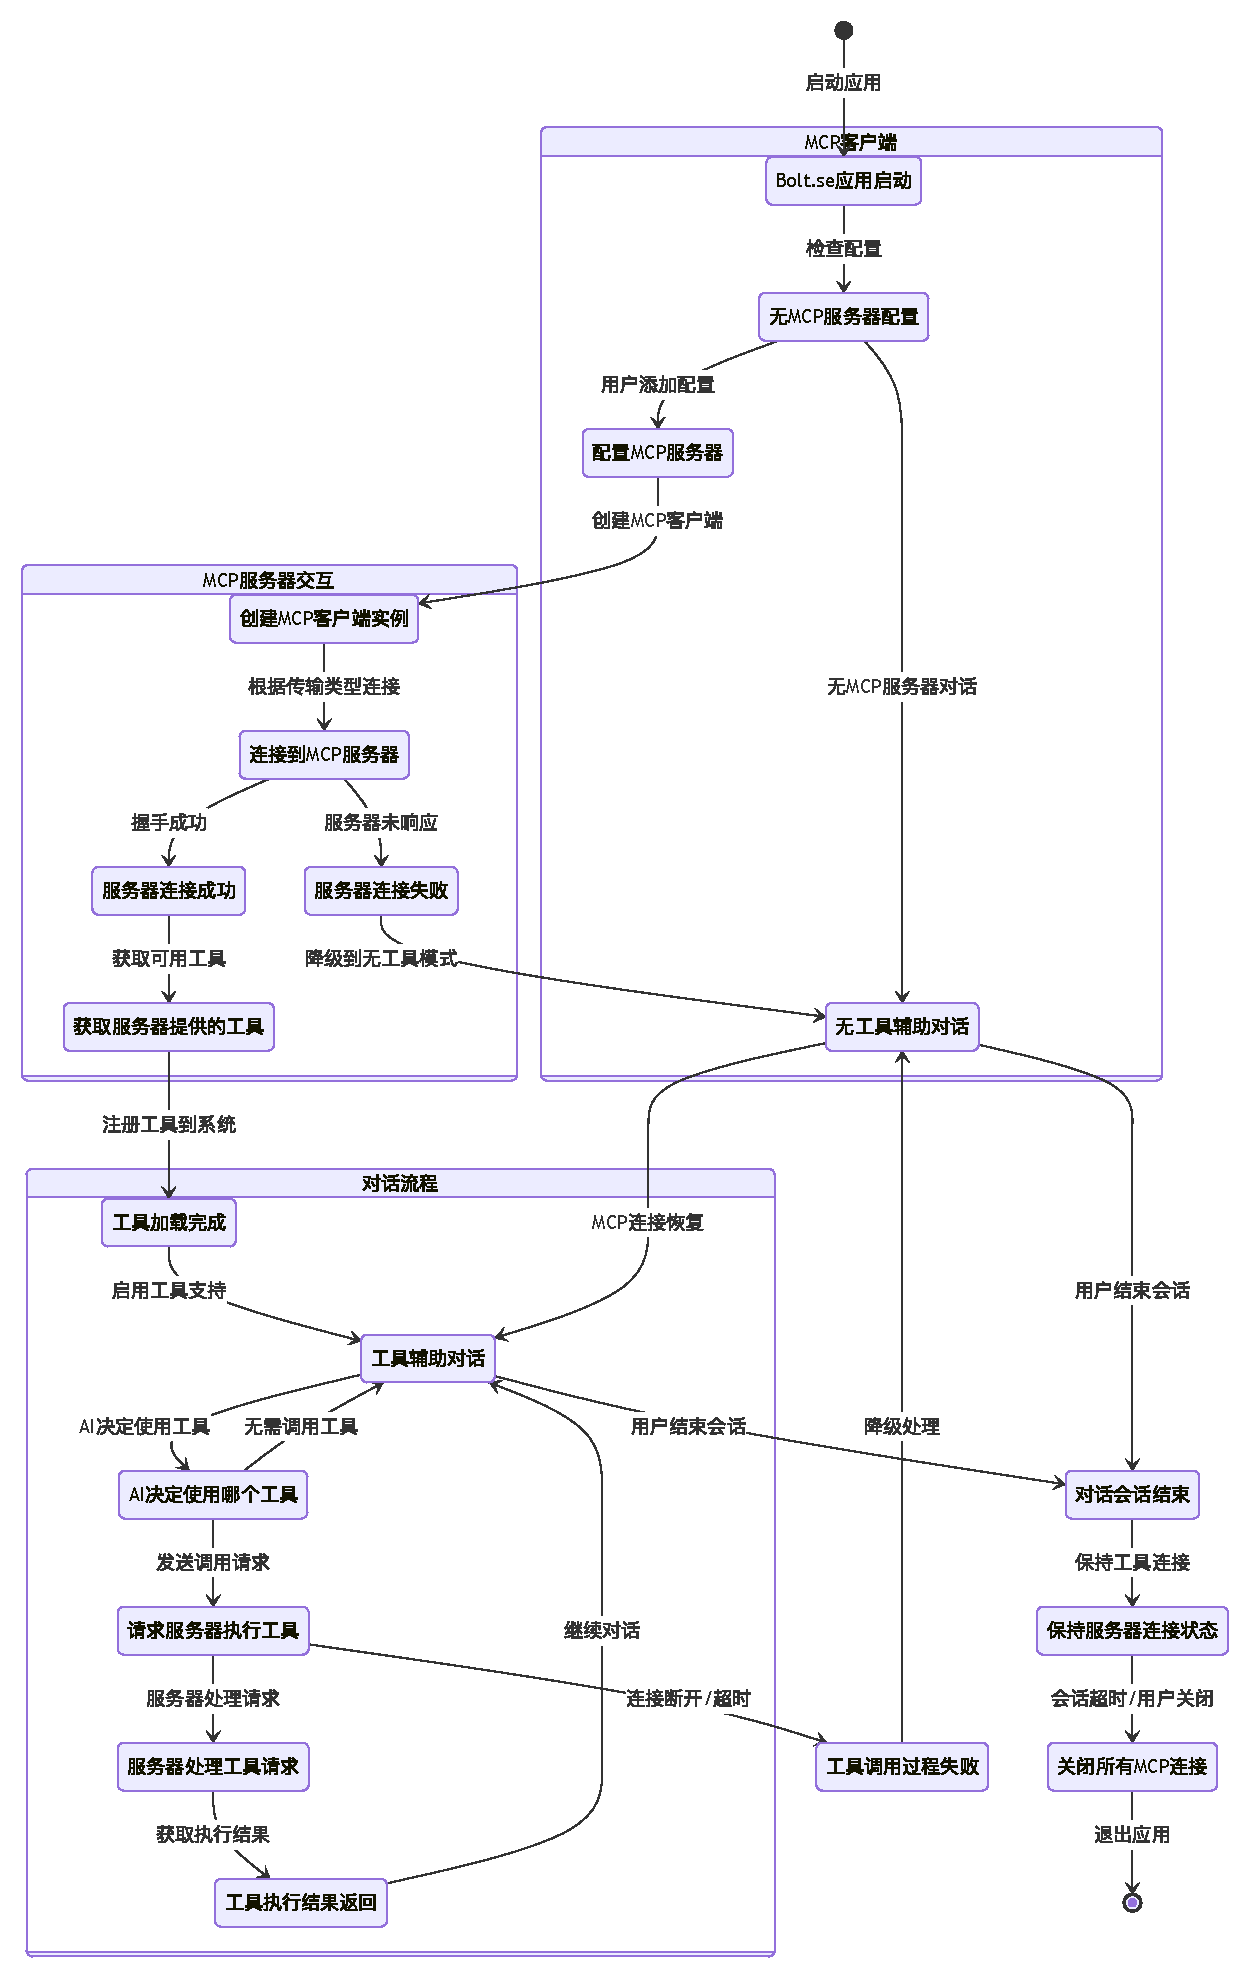
\includegraphics[width=\textwidth]{figures/mcp_state.pdf}
  \caption{MCP状态图:描述了MCP连接的各个状态及其转换关系,从初始配置到工具调用的完整流程}
  \label{fig:mcp_state}
\end{figure}

% stateDiagram-v2
%     [*] --> Host初始状态 : 启动应用
    
%     state MCP客户端 {
%         Host初始状态 --> 未配置 : 检查配置
%         未配置 --> 配置中 : 用户添加配置
%         未配置 --> 基础对话模式 : 无MCP服务器对话
%         配置中 --> 连接初始化 : 创建MCP客户端
%     }
    
%     state MCP服务器交互 {
%         连接初始化 --> 服务器连接中 : 根据传输类型连接
%         服务器连接中 --> 连接失败 : 服务器未响应
%         服务器连接中 --> 连接成功 : 握手成功
%         连接成功 --> 工具发现 : 获取可用工具
%         工具发现 --> 工具就绪 : 注册工具到系统
%     }
    
%     state 对话流程 {
%         工具就绪 --> 增强对话模式 : 启用工具支持
%         增强对话模式 --> 工具选择 : AI决定使用工具
%         工具选择 --> 工具调用 : 发送调用请求
%         工具调用 --> 工具执行 : 服务器处理请求
%         工具执行 --> 结果返回 : 获取执行结果
%         结果返回 --> 增强对话模式 : 继续对话
%         工具选择 --> 增强对话模式 : 无需调用工具
%     }
    
%     连接失败 --> 基础对话模式 : 降级到无工具模式
%     基础对话模式 --> 增强对话模式 : MCP连接恢复
    
%     增强对话模式 --> 会话结束 : 用户结束会话
%     基础对话模式 --> 会话结束 : 用户结束会话
    
%     工具调用 --> 调用失败 : 连接断开/超时
%     调用失败 --> 基础对话模式 : 降级处理
    
%     会话结束 --> 连接保持 : 保持工具连接
%     连接保持 --> 连接关闭 : 会话超时/用户关闭
%     连接关闭 --> [*] : 退出应用
    
%     Host初始状态 : Bolt.se应用启动
%     未配置 : 无MCP服务器配置
%     配置中 : 配置MCP服务器
%     连接初始化 : 创建MCP客户端实例
%     服务器连接中 : 连接到MCP服务器
%     连接失败 : 服务器连接失败
%     连接成功 : 服务器连接成功
%     工具发现 : 获取服务器提供的工具
%     工具就绪 : 工具加载完成
%     基础对话模式 : 无工具辅助对话
%     增强对话模式 : 工具辅助对话
%     工具选择 : AI决定使用哪个工具
%     工具调用 : 请求服务器执行工具
%     工具执行 : 服务器处理工具请求
%     结果返回 : 工具执行结果返回
%     调用失败 : 工具调用过程失败
%     会话结束 : 对话会话结束
%     连接保持 : 保持服务器连接状态
%     连接关闭 : 关闭所有MCP连接 

如图\ref{fig:mcp_state}所示,MCP连接的生命周期可分为四个主要阶段:MCP客户端初始化、MCP服务器交互、对话流程和会话结束。在应用启动后,系统首先检查MCP配置,若配置存在则创建相应MCP客户端并尝试连接服务器。连接成功后,系统进入工具发现阶段,获取服务器提供的工具并将其注册到系统中。当工具就绪后,用户对话转入增强模式,LLM能够根据需要选择并调用工具,处理各种复杂任务。状态图还展示了错误处理机制:当连接失败或工具调用出错时,系统会降级到基础对话模式,确保用户体验不中断。最后,当用户结束会话时,系统会根据配置决定是保持连接还是关闭所有MCP客户端。这种设计确保了bolt.se中MCP功能的健壮性和可靠性,能够优雅地处理各种正常和异常情况。

在数据模型设计方面,bolt.se定义了结构化的MCP配置数据模型:

\begin{enumerate}
  \item \textbf{MCPConfig}:顶层配置对象,包含服务器映射表
  
  \item \textbf{ServerConfig}:服务器配置对象,根据传输类型包含不同的属性:
    \begin{itemize}
      \item \textit{stdio配置}:包括命令(command)、参数(args)、环境变量(env)和工作目录(cwd)
      \item \textit{SSE配置}:包括URL(url)和类型(type)
    \end{itemize}
  
  \item \textbf{MCPClient}:客户端接口,定义了获取工具(tools)和关闭连接(close)的方法
\end{enumerate}

bolt.se的MCP模块设计充分考虑了灵活性和扩展性,支持多种MCP服务器类型,并能够动态发现和整合它们提供的工具。

\subsection{服务器配置与连接管理}
bolt.se实现了强大的MCP服务器配置和连接管理功能,使用户能够灵活地添加和管理不同类型的MCP服务器:

\begin{enumerate}
  \item \textbf{配置存储}:使用IndexedDB持久化存储MCP配置,确保配置在页面刷新和会话之间保持一致:
    \begin{itemize}
      \item \texttt{saveMCPConfig}:将配置保存到数据库
      \item \texttt{getMCPConfig}:从数据库获取配置
      \item \texttt{deleteMCPConfig}:删除配置
    \end{itemize}
  
  \item \textbf{配置管理Hook}:提供\texttt{useMCPConfig} React Hook,封装配置管理逻辑,包括:
    \begin{itemize}
      \item 加载和初始化配置
      \item 更新配置并保存到存储
      \item 配置变更事件通知
    \end{itemize}
  
  \item \textbf{服务器连接检查}:实现服务器可用性检查机制,验证配置的有效性:
    \begin{itemize}
      \item 尝试连接到每个配置的服务器
      \item 获取可用工具列表
      \item 报告连接状态和错误信息
    \end{itemize}
  
  \item \textbf{配置界面}:提供友好的用户界面,用于查看和编辑MCP配置:
    \begin{itemize}
      \item JSON编辑器,支持直接编辑配置
      \item 服务器状态指示器,显示每个服务器的可用性
      \item 工具浏览器,展示每个服务器提供的工具及其模式
    \end{itemize}
\end{enumerate}

这些功能使用户能够轻松管理MCP服务器配置,验证其可用性,并了解可用的工具集,为AI辅助开发提供强大的扩展能力。

\subsection{MCP客户端实现与工具集成}
bolt.se实现了灵活的MCP客户端创建和工具集成机制:

\begin{enumerate}
  \item \textbf{客户端工厂}:\texttt{createMCPClient}函数根据服务器配置创建适当类型的MCP客户端:
    \begin{itemize}
      \item 对于stdio类型,创建基于子进程的客户端
      \item 对于SSE类型,创建基于HTTP连接的客户端
    \end{itemize}
  
  \item \textbf{客户端管理}:\texttt{createMCPClients}函数管理多个MCP客户端:
    \begin{itemize}
      \item 并行创建多个服务器的客户端
      \item 收集和合并所有客户端提供的工具
      \item 处理连接错误,确保部分服务器失败不影响整体功能
    \end{itemize}
  
  \item \textbf{工具发现}:通过客户端的\texttt{tools}方法获取服务器提供的工具:
    \begin{itemize}
      \item 解析工具模式,包括名称、描述和参数
      \item 创建工具的JavaScript表示,供LLM调用
    \end{itemize}
  
  \item \textbf{LLM集成}:将MCP工具集成到LLM的对话上下文中:
    \begin{itemize}
      \item 在AI请求中包含工具定义
      \item 处理LLM的工具调用请求
      \item 执行工具操作并返回结果
      \item 将结果整合回对话流
    \end{itemize}
  
  \item \textbf{资源清理}:\texttt{closeMCPClients}函数确保正确关闭所有MCP客户端:
    \begin{itemize}
      \item 在对话结束或页面卸载时关闭连接
      \item 处理关闭过程中的错误
    \end{itemize}
\end{enumerate}

这种实现使bolt.se能够无缝集成多种MCP服务器提供的工具,大大增强了LLM的功能范围和问题解决能力。

\begin{figure}[htbp]
  \centering
  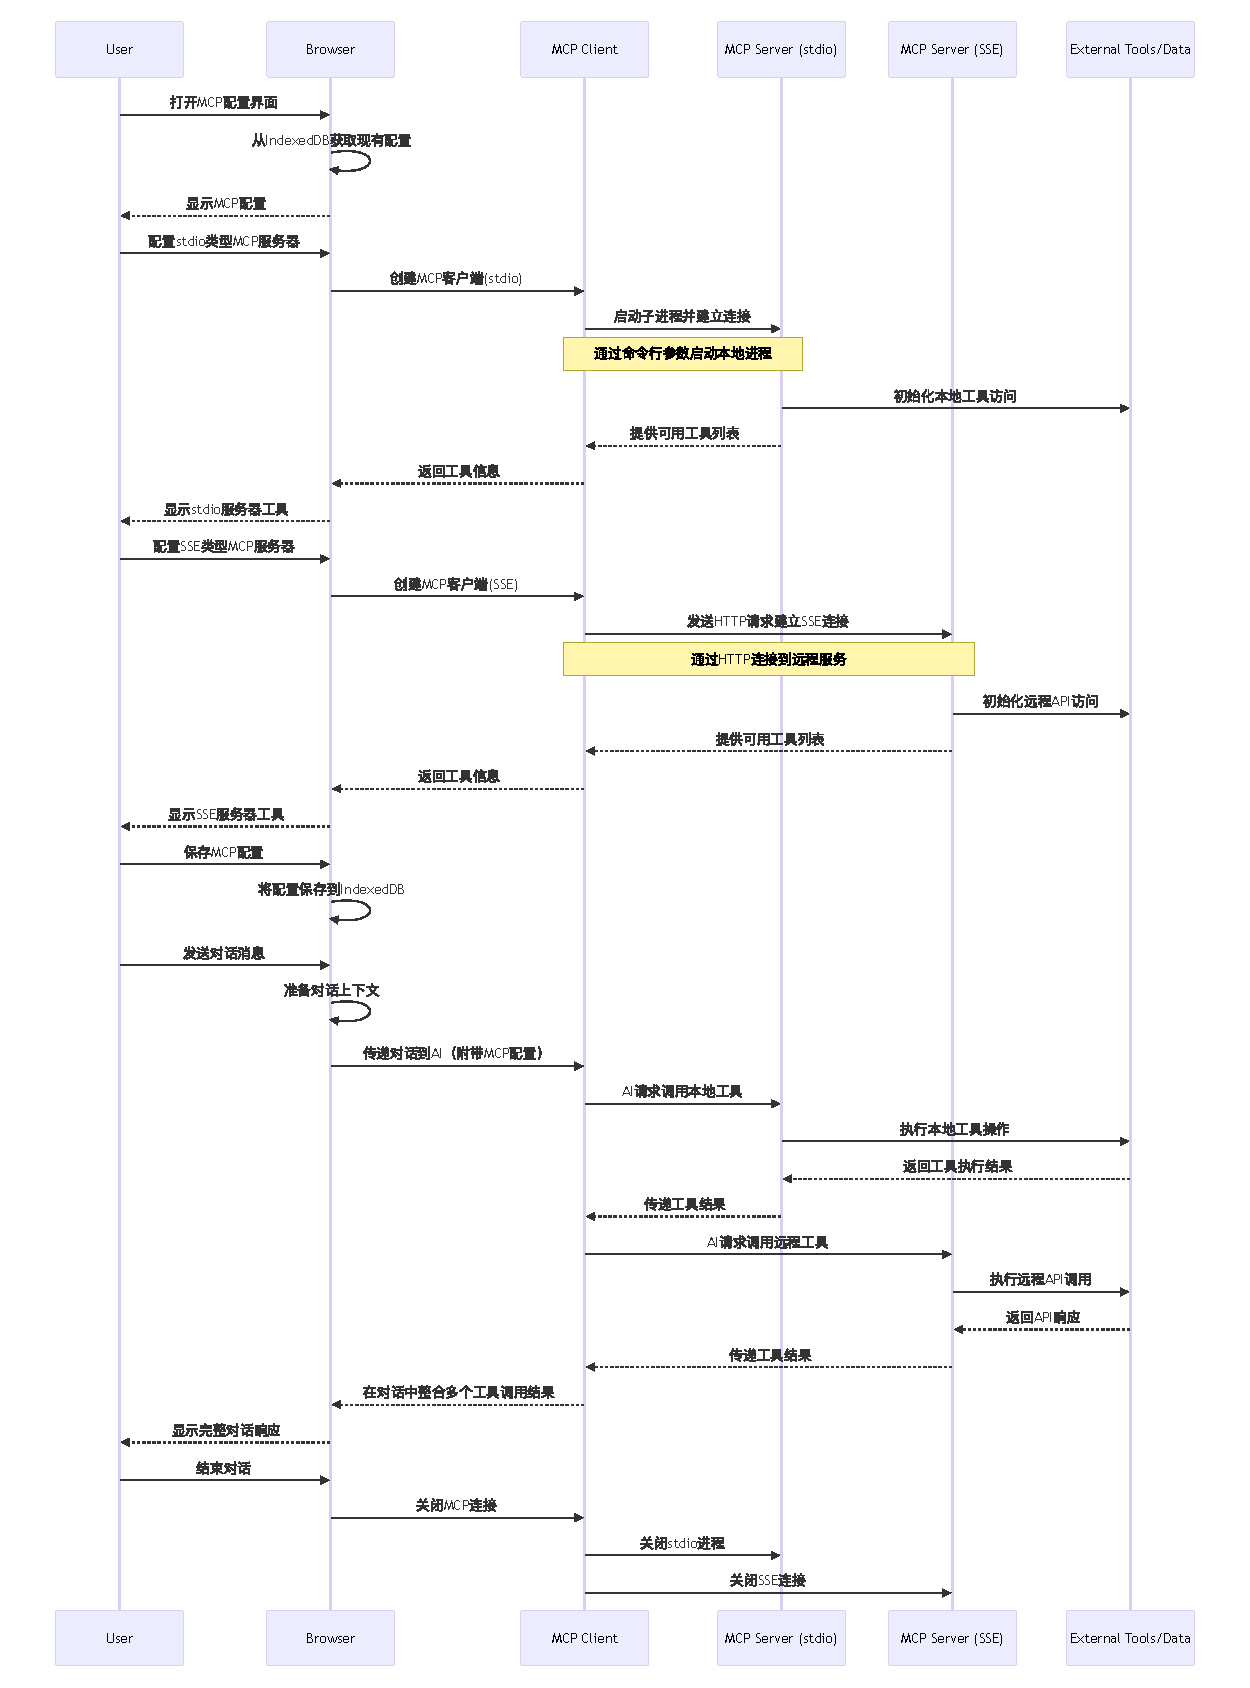
\includegraphics[width=\textwidth]{figures/mcp_sequence.pdf}
  \caption{MCP序列图:展示了用户、客户端和不同类型服务器之间的交互序列,包括配置、连接和工具调用过程}
  \label{fig:mcp_sequence}
\end{figure}

% sequenceDiagram
%     participant User
%     participant Host as Browser
%     participant Client as MCP Client
%     participant ServerStdio as MCP Server (stdio)
%     participant ServerSSE as MCP Server (SSE)
%     participant Tools as External Tools/Data

%     %% 配置过程
%     User->>Host: 打开MCP配置界面
%     Host->>Host: 从IndexedDB获取现有配置
%     Host-->>User: 显示MCP配置
    
%     %% stdio方式配置
%     User->>Host: 配置stdio类型MCP服务器
%     Host->>Client: 创建MCP客户端(stdio)
%     Client->>ServerStdio: 启动子进程并建立连接
%     Note over Client,ServerStdio: 通过命令行参数启动本地进程
%     ServerStdio->>Tools: 初始化本地工具访问
%     ServerStdio-->>Client: 提供可用工具列表
%     Client-->>Host: 返回工具信息
%     Host-->>User: 显示stdio服务器工具
    
%     %% SSE方式配置
%     User->>Host: 配置SSE类型MCP服务器
%     Host->>Client: 创建MCP客户端(SSE)
%     Client->>ServerSSE: 发送HTTP请求建立SSE连接
%     Note over Client,ServerSSE: 通过HTTP连接到远程服务
%     ServerSSE->>Tools: 初始化远程API访问
%     ServerSSE-->>Client: 提供可用工具列表
%     Client-->>Host: 返回工具信息
%     Host-->>User: 显示SSE服务器工具
    
%     %% 保存配置
%     User->>Host: 保存MCP配置
%     Host->>Host: 将配置保存到IndexedDB
    
%     %% 对话过程
%     User->>Host: 发送对话消息
%     Host->>Host: 准备对话上下文
    
%     %% 根据配置选择传输方式
%     Host->>Client: 传递对话到AI(附带MCP配置)
    
%     %% 通过stdio调用工具
%     Client->>ServerStdio: AI请求调用本地工具
%     ServerStdio->>Tools: 执行本地工具操作
%     Tools-->>ServerStdio: 返回工具执行结果
%     ServerStdio-->>Client: 传递工具结果
    
%     %% 通过SSE调用工具
%     Client->>ServerSSE: AI请求调用远程工具
%     ServerSSE->>Tools: 执行远程API调用
%     Tools-->>ServerSSE: 返回API响应
%     ServerSSE-->>Client: 传递工具结果
    
%     %% 结果整合
%     Client-->>Host: 在对话中整合多个工具调用结果
%     Host-->>User: 显示完整对话响应

%     %% 会话结束
%     User->>Host: 结束对话
%     Host->>Client: 关闭MCP连接
%     Client->>ServerStdio: 关闭stdio进程
%     Client->>ServerSSE: 关闭SSE连接 

如图\ref{fig:mcp_sequence}所示,序列图详细展示了用户、浏览器(Host)、MCP客户端以及不同类型服务器(stdio和SSE)之间的完整交互流程。图中首先描述了配置阶段:用户通过界面配置MCP服务器,包括本地stdio服务器和远程SSE服务器的初始化过程。对于stdio类型服务器,系统通过命令行参数启动本地进程;而对于SSE类型服务器,则通过HTTP建立远程连接。两种服务器初始化后都会返回可用工具列表,并在Host端显示给用户。在对话阶段,当用户发送消息时,系统根据配置将请求路由到相应的MCP服务器,执行工具操作并获取结果。最后在会话结束时,系统会妥善关闭所有连接,释放资源。这一序列图清晰地展示了MCP在不同传输模式下的完整生命周期,以及各组件之间的紧密协作关系,体现了bolt.se中MCP实现的灵活性和完整性。

\section{MCP在bolt.se中的应用场景}

bolt.se中的MCP实现支持多种应用场景,从本地工具集成到云服务接入。本节通过具体实例,展示MCP如何增强bolt.se的功能,为用户提供更强大的AI辅助开发体验。

\subsection{本地文件系统访问}

使用stdio类型MCP服务器,bolt.se可以安全地访问本地文件系统,执行文件操作:

\begin{verbatim}
{
  "mcpServers": {
    "localFiles": {
      "type": "stdio",
      "command": "node",
      "args": ["./mcp-file-server.js"]
    }
  }
}
\end{verbatim}

这种配置使LLM能够:
\begin{itemize}
  \item 读取本地文件内容,理解项目结构和代码
  \item 创建新文件,实现代码生成和文档创建
  \item 修改和更新文件,进行代码重构和优化
  \item 导航和搜索文件系统,查找相关资源
\end{itemize}

用户可以通过自然语言指令,让LLM访问和操作本地文件,如"分析项目结构并提供改进建议"、"创建新的组件文件"等。

\subsection{外部API集成}

使用SSE类型MCP服务器,bolt.se可以集成外部API和云服务:

\begin{verbatim}
{
  "mcpServers": {
    "weatherAPI": {
      "type": "sse",
      "url": "https://weather-mcp.example.com/connect"
    },
    "databaseAccess": {
      "type": "sse",
      "url": "https://db-mcp.example.com/connect"
    }
  }
}
\end{verbatim}

这种配置使LLM能够:
\begin{itemize}
  \item 获取实时数据,如天气信息、股票价格等
  \item 访问在线数据库,查询和更新数据
  \item 调用专业服务API,如翻译、图像分析等
  \item 与企业内部系统集成,访问业务数据和流程
\end{itemize}

用户可以通过自然语言指令,让LLM调用这些API,如"获取纽约的天气预报"、"查询产品销售数据并生成分析报告"等。

\subsection{开发工具集成}

使用专用MCP服务器,bolt.se可以集成各种开发工具:

\begin{verbatim}
{
  "mcpServers": {
    "gitOperations": {
      "type": "stdio",
      "command": "node",
      "args": ["./mcp-git-server.js"]
    },
    "codeAnalysis": {
      "type": "sse",
      "url": "https://code-analysis-mcp.example.com/connect"
    }
  }
}
\end{verbatim}

这种配置使LLM能够:
\begin{itemize}
  \item 执行Git操作,如克隆、提交、分支管理等
  \item 运行代码分析工具,检测问题和优化机会
  \item 执行构建和测试流程,验证代码质量
  \item 部署应用到开发环境,测试实际效果
\end{itemize}

用户可以通过自然语言指令,让LLM使用这些开发工具,如"创建新分支并提交这些变更"、"分析代码质量并修复问题"等。

\section{MCP与传统AI开发方式对比}

MCP方式与传统AI开发方式相比具有显著优势:

\begin{enumerate}
  \item \textbf{功能扩展}:传统AI模型受限于训练数据和内置功能,而MCP通过工具集成极大扩展了功能边界,使AI能够执行原本不可能的任务。

  \item \textbf{实时性与准确性}:传统模型依赖训练时的知识,而MCP使模型能够访问最新数据和专业工具,提供更准确、更实时的结果。

  \item \textbf{开发效率}:传统方式需要针对每个新需求更新模型,而MCP允许通过添加新工具扩展功能,大大提高了开发效率和迭代速度。

  \item \textbf{资源优化}:传统模型需要更大的参数规模来涵盖更多功能,而MCP通过专用工具分担任务,优化了计算资源使用。

  \item \textbf{安全性与控制}:传统模型可能产生不可预测的输出,而MCP提供了明确的功能边界和权限控制,增强了安全性和可靠性。
\end{enumerate}

在bolt.se中,MCP的优势使其成为连接AI和外部世界的理想桥梁,为用户提供了安全、灵活且功能强大的开发环境。通过MCP,bolt.se能够将LLM的创造力与专业工具的精确性结合起来,创造超越传统AI应用的用户体验。

\section{实例应用场景}
\label{sec:mcp-iotdb-demo}

本节以 "\textbf{通过 MCP 协同 IoTDB 与 OpenAPI 自动生成可交互前端应用}" 为例,说明
\begin{enumerate}
  \item 如何将时序数据库 \textit{Apache IoTDB} 暴露为两类外部能力:\textbf{MCP 工具} 与 \textbf{REST API};
  \item bolt.se 如何在一次自然语言提示中同时发现并调用两类能力;
  \item LLM 如何根据实时查询结果快速产出可视化应用,并通过 \textit{Reload} 按钮实现数据刷新。
\end{enumerate}

\subsection{场景概述}

开发者使用表格方言 (\texttt{table}) 在本地部署 \texttt{IoTDB 2.0.2},
并将名为 \texttt{battery\_data} 的示例表写入 30 条监测数据(电压、电流等)。
随后分两条通路暴露数据库能力:

\begin{enumerate}
  \item \textbf{MCP 通路}——借助 \texttt{remote-sse} 服务器,将
        \textit{list\_tables}、\textit{describe\_table} 与
        \textit{read\_query} 三个工具提供给 LLM;
  \item \textbf{REST 通路}——通过 IoTDB 自带 REST Service V2,把
        查询接口 \texttt{/rest/table/v1/query} 描述成 OpenAPI 3.0 规范。
\end{enumerate}

\subsection{MCP 服务器配置(工具发现)}

图~\ref{fig:mcp-config} 展示了在 bolt.se
\textit{MCP Configuration} 面板中填入如下 JSON 并点击
\textit{Check availability} 后,系统成功探测到
\texttt{read\_query} 等三项工具并给出 "Available" 反馈:

\begin{verbatim}
{
  "mcpServers": {
    "remote-sse": {
      "type": "sse",
      "url": "http://localhost:8000/sse"
    }
  }
}
\end{verbatim}

\begin{figure}[htbp]
  \centering
  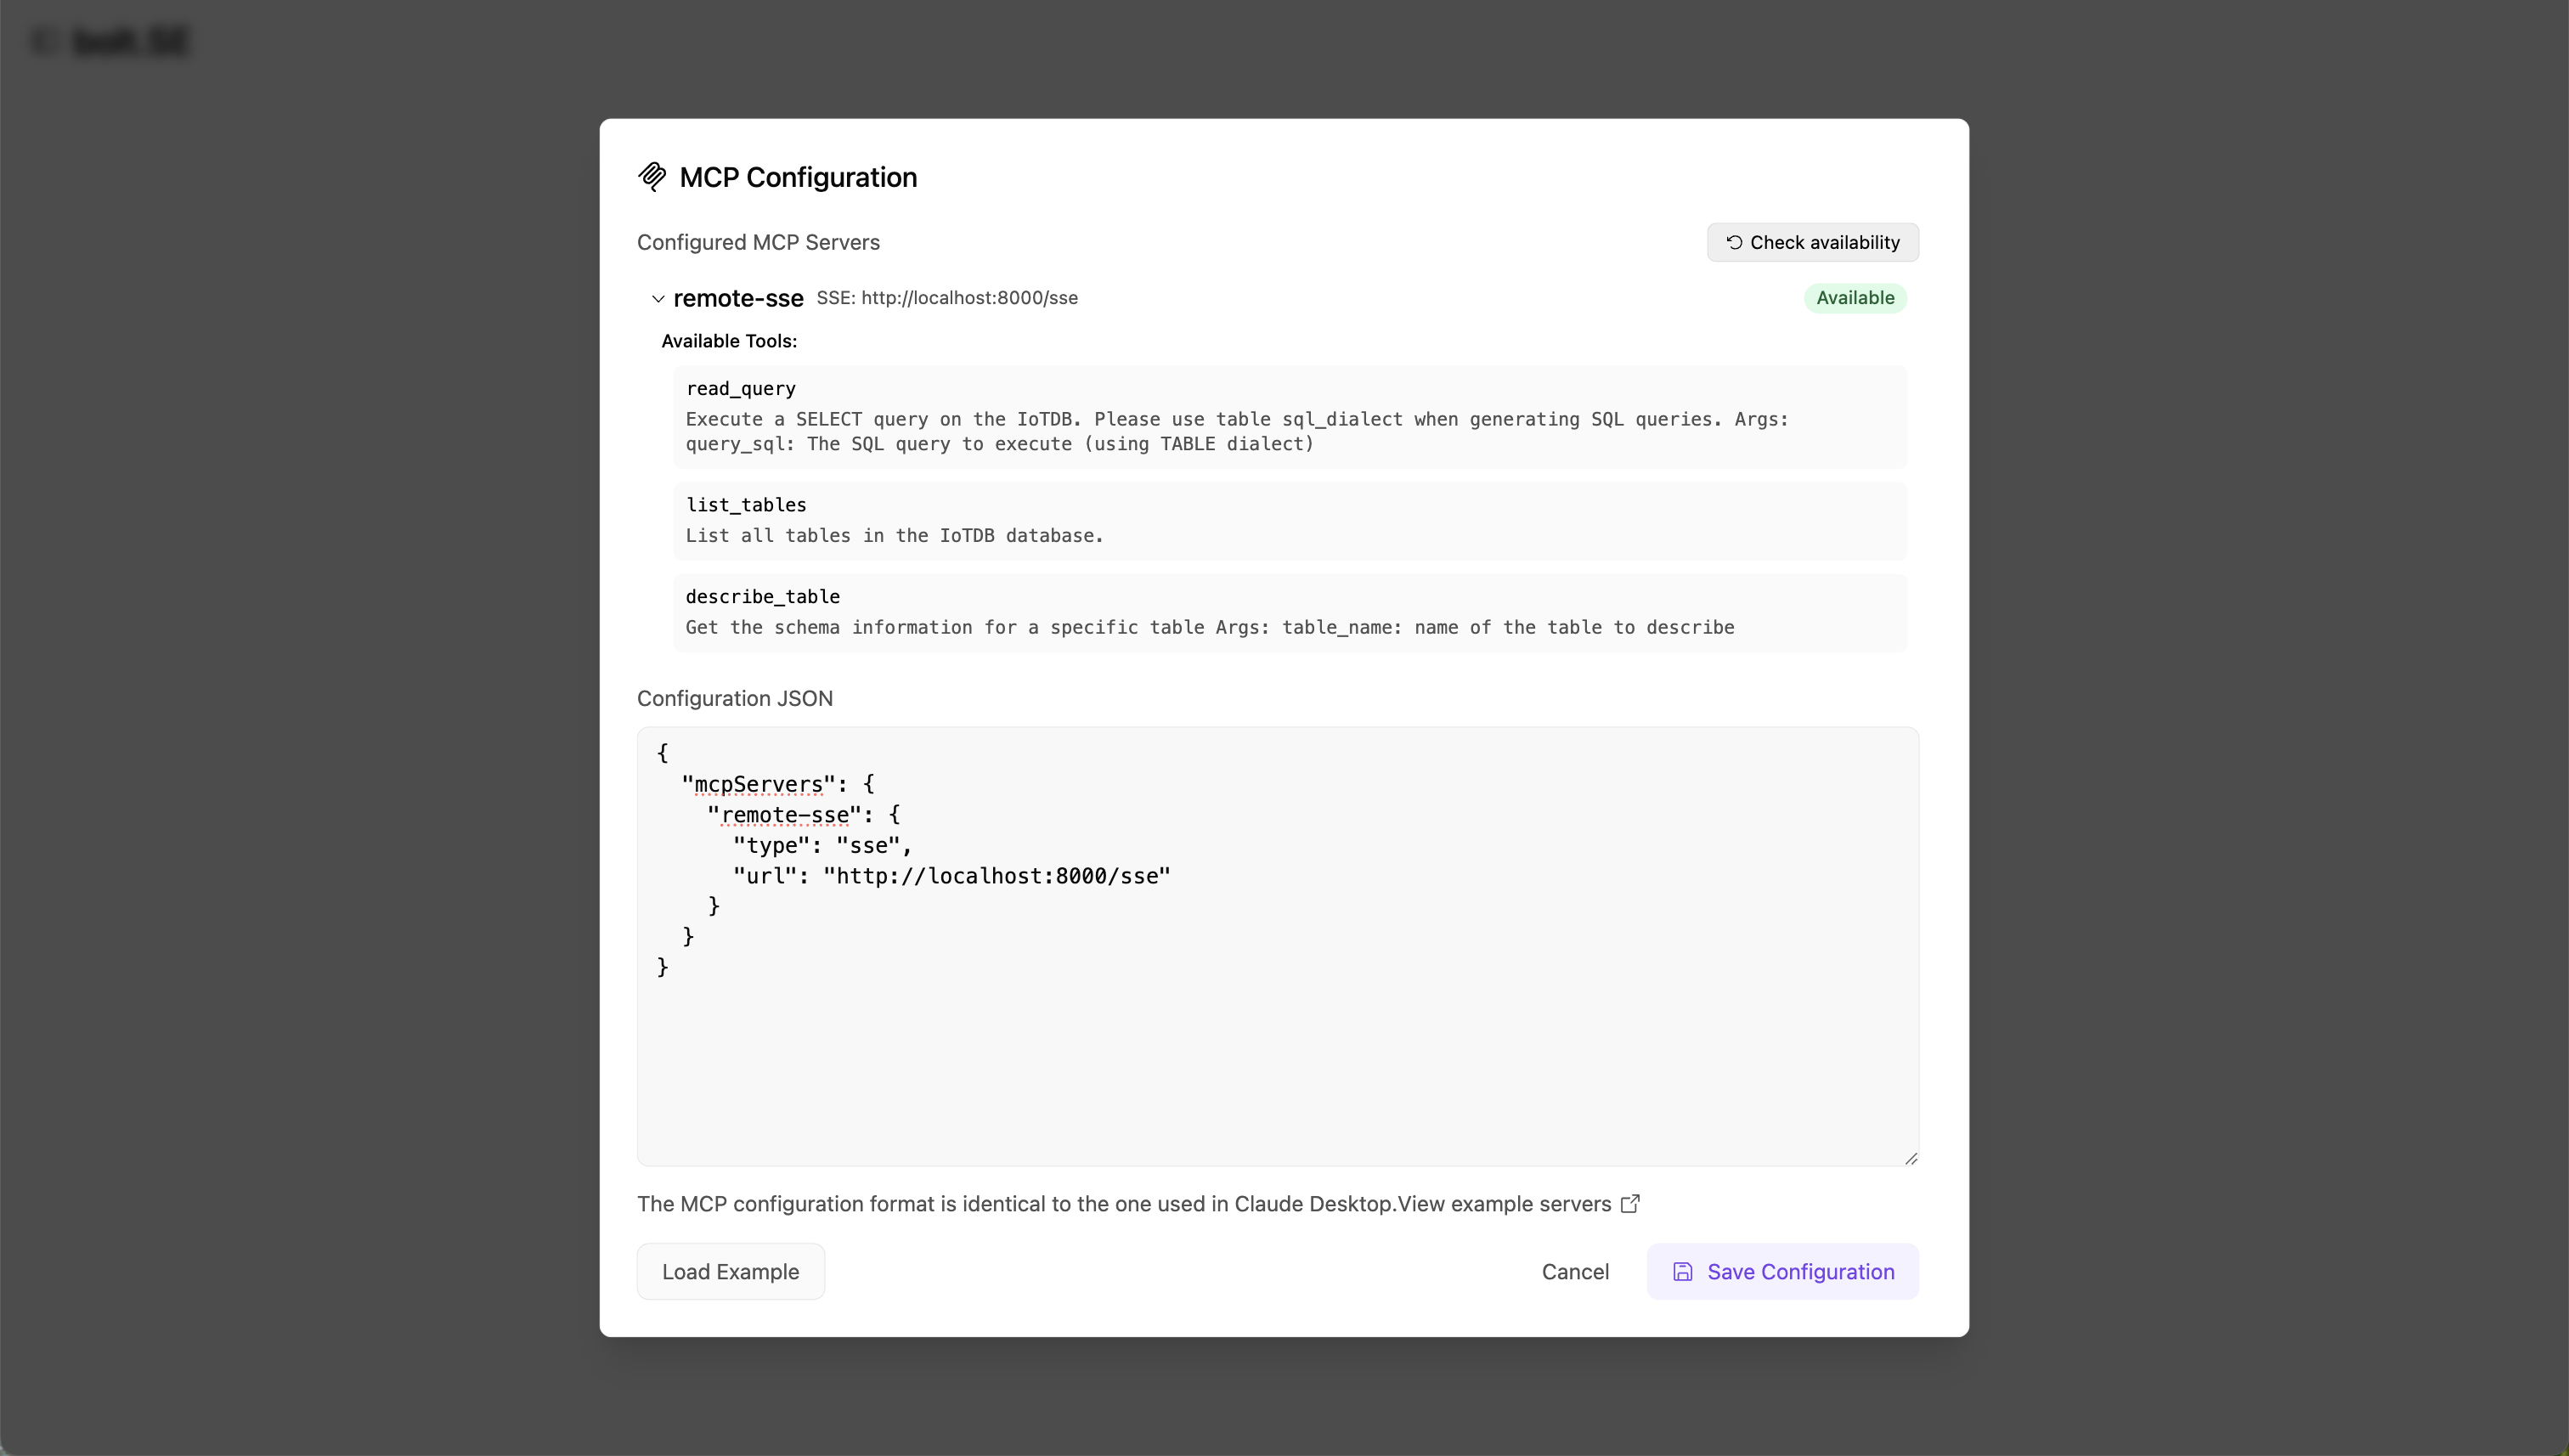
\includegraphics[width=.7\textwidth]{figures/screenshots/iotdb-demo/mcp-config.png}
  \caption{配置 \texttt{remote-sse} 并成功发现三项 IoTDB 工具}
  \label{fig:mcp-config}
\end{figure}

\subsection{REST API 规范与动作注册}

开发者将 IoTDB 查询接口写成 OpenAPI 3.0 文档
(见下面摘录),并在
\textit{Edit actions} 弹窗里粘贴、指定 \texttt{Basic}
认证头 \verb|cm9vdDpyb290|。  
图~\ref{fig:openapi-editor} 展示了编辑过程,图~\ref{fig:api-actions}
展示了最终动作列表,仅保留 \textit{queryTableData} 一项。

\begin{verbatim}
paths:
  /rest/table/v1/query:
    post:
      operationId: queryTableData
      summary: Execute a SQL query on the IoTDB table
      requestBody:
        required: true
        content:
          application/json:
            schema:
              type: object
              required: [database, sql]
\end{verbatim}

\begin{figure}[htbp]
  \centering
  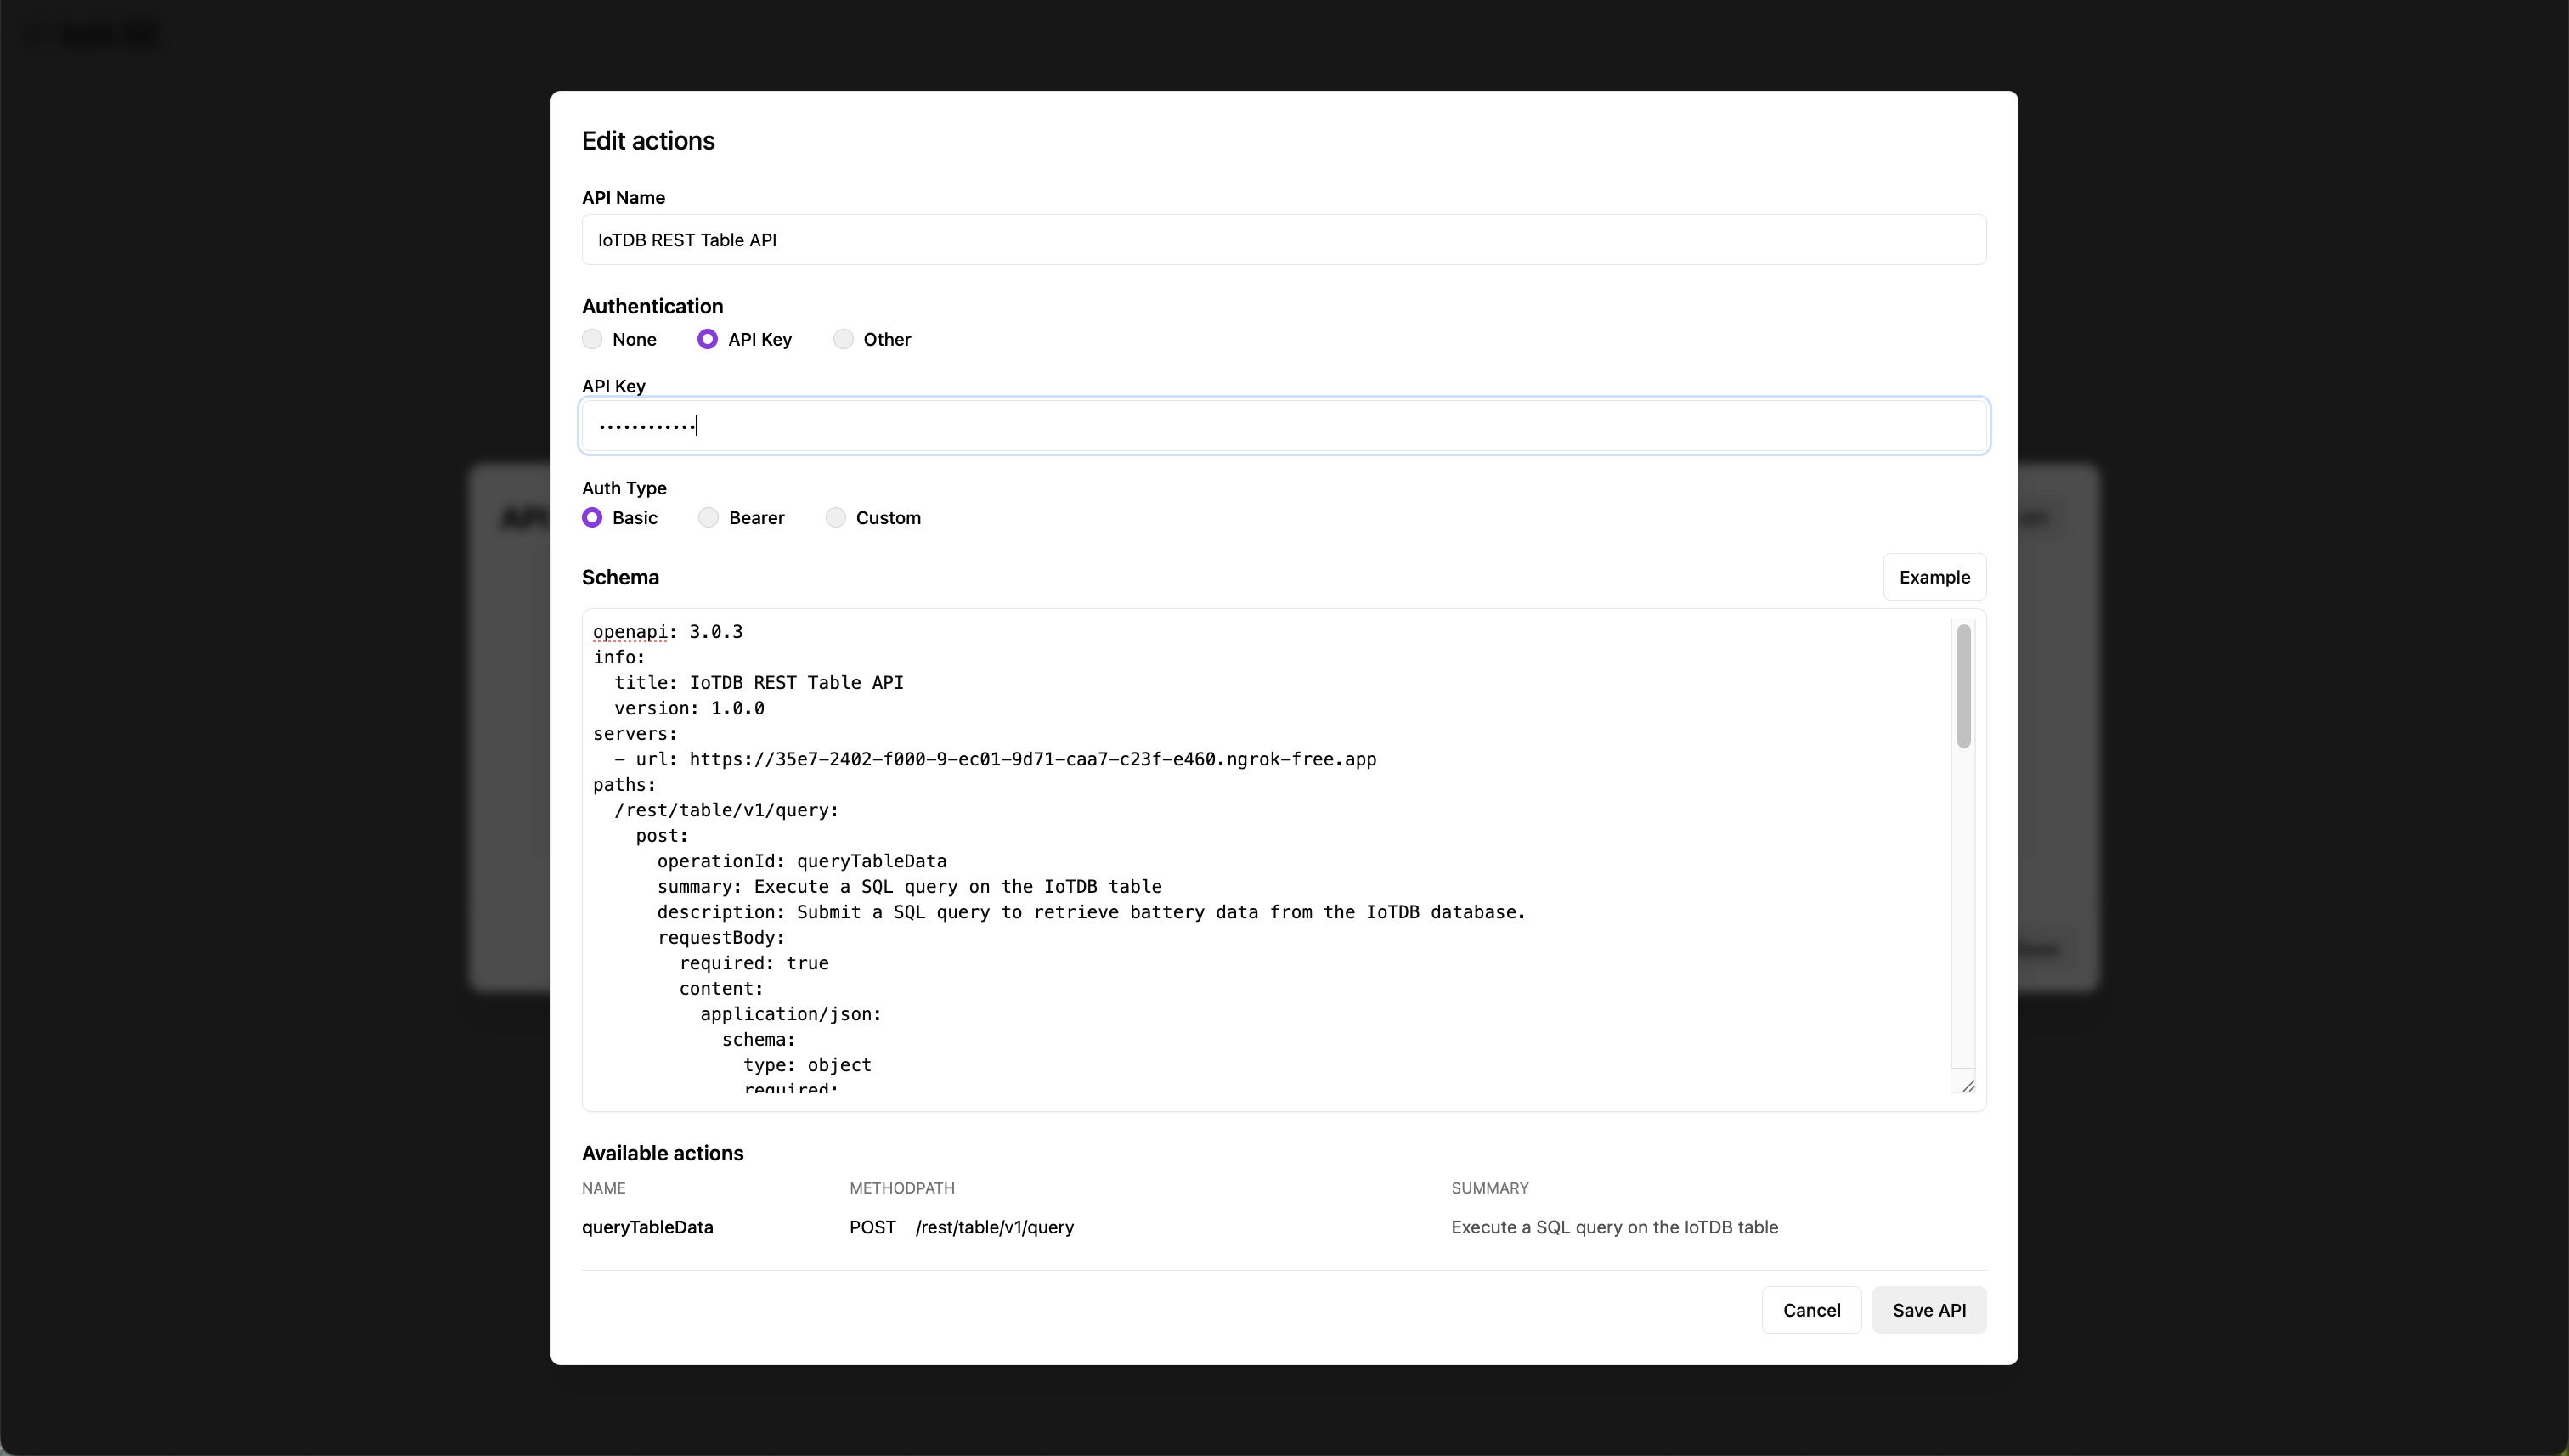
\includegraphics[width=.7\textwidth]{figures/screenshots/iotdb-demo/openapi-editor.png}
  \caption{在 \textit{Edit actions} 对话框中粘贴 OpenAPI 文档并填入认证信息}
  \label{fig:openapi-editor}
\end{figure}

\begin{figure}[htbp]
  \centering
  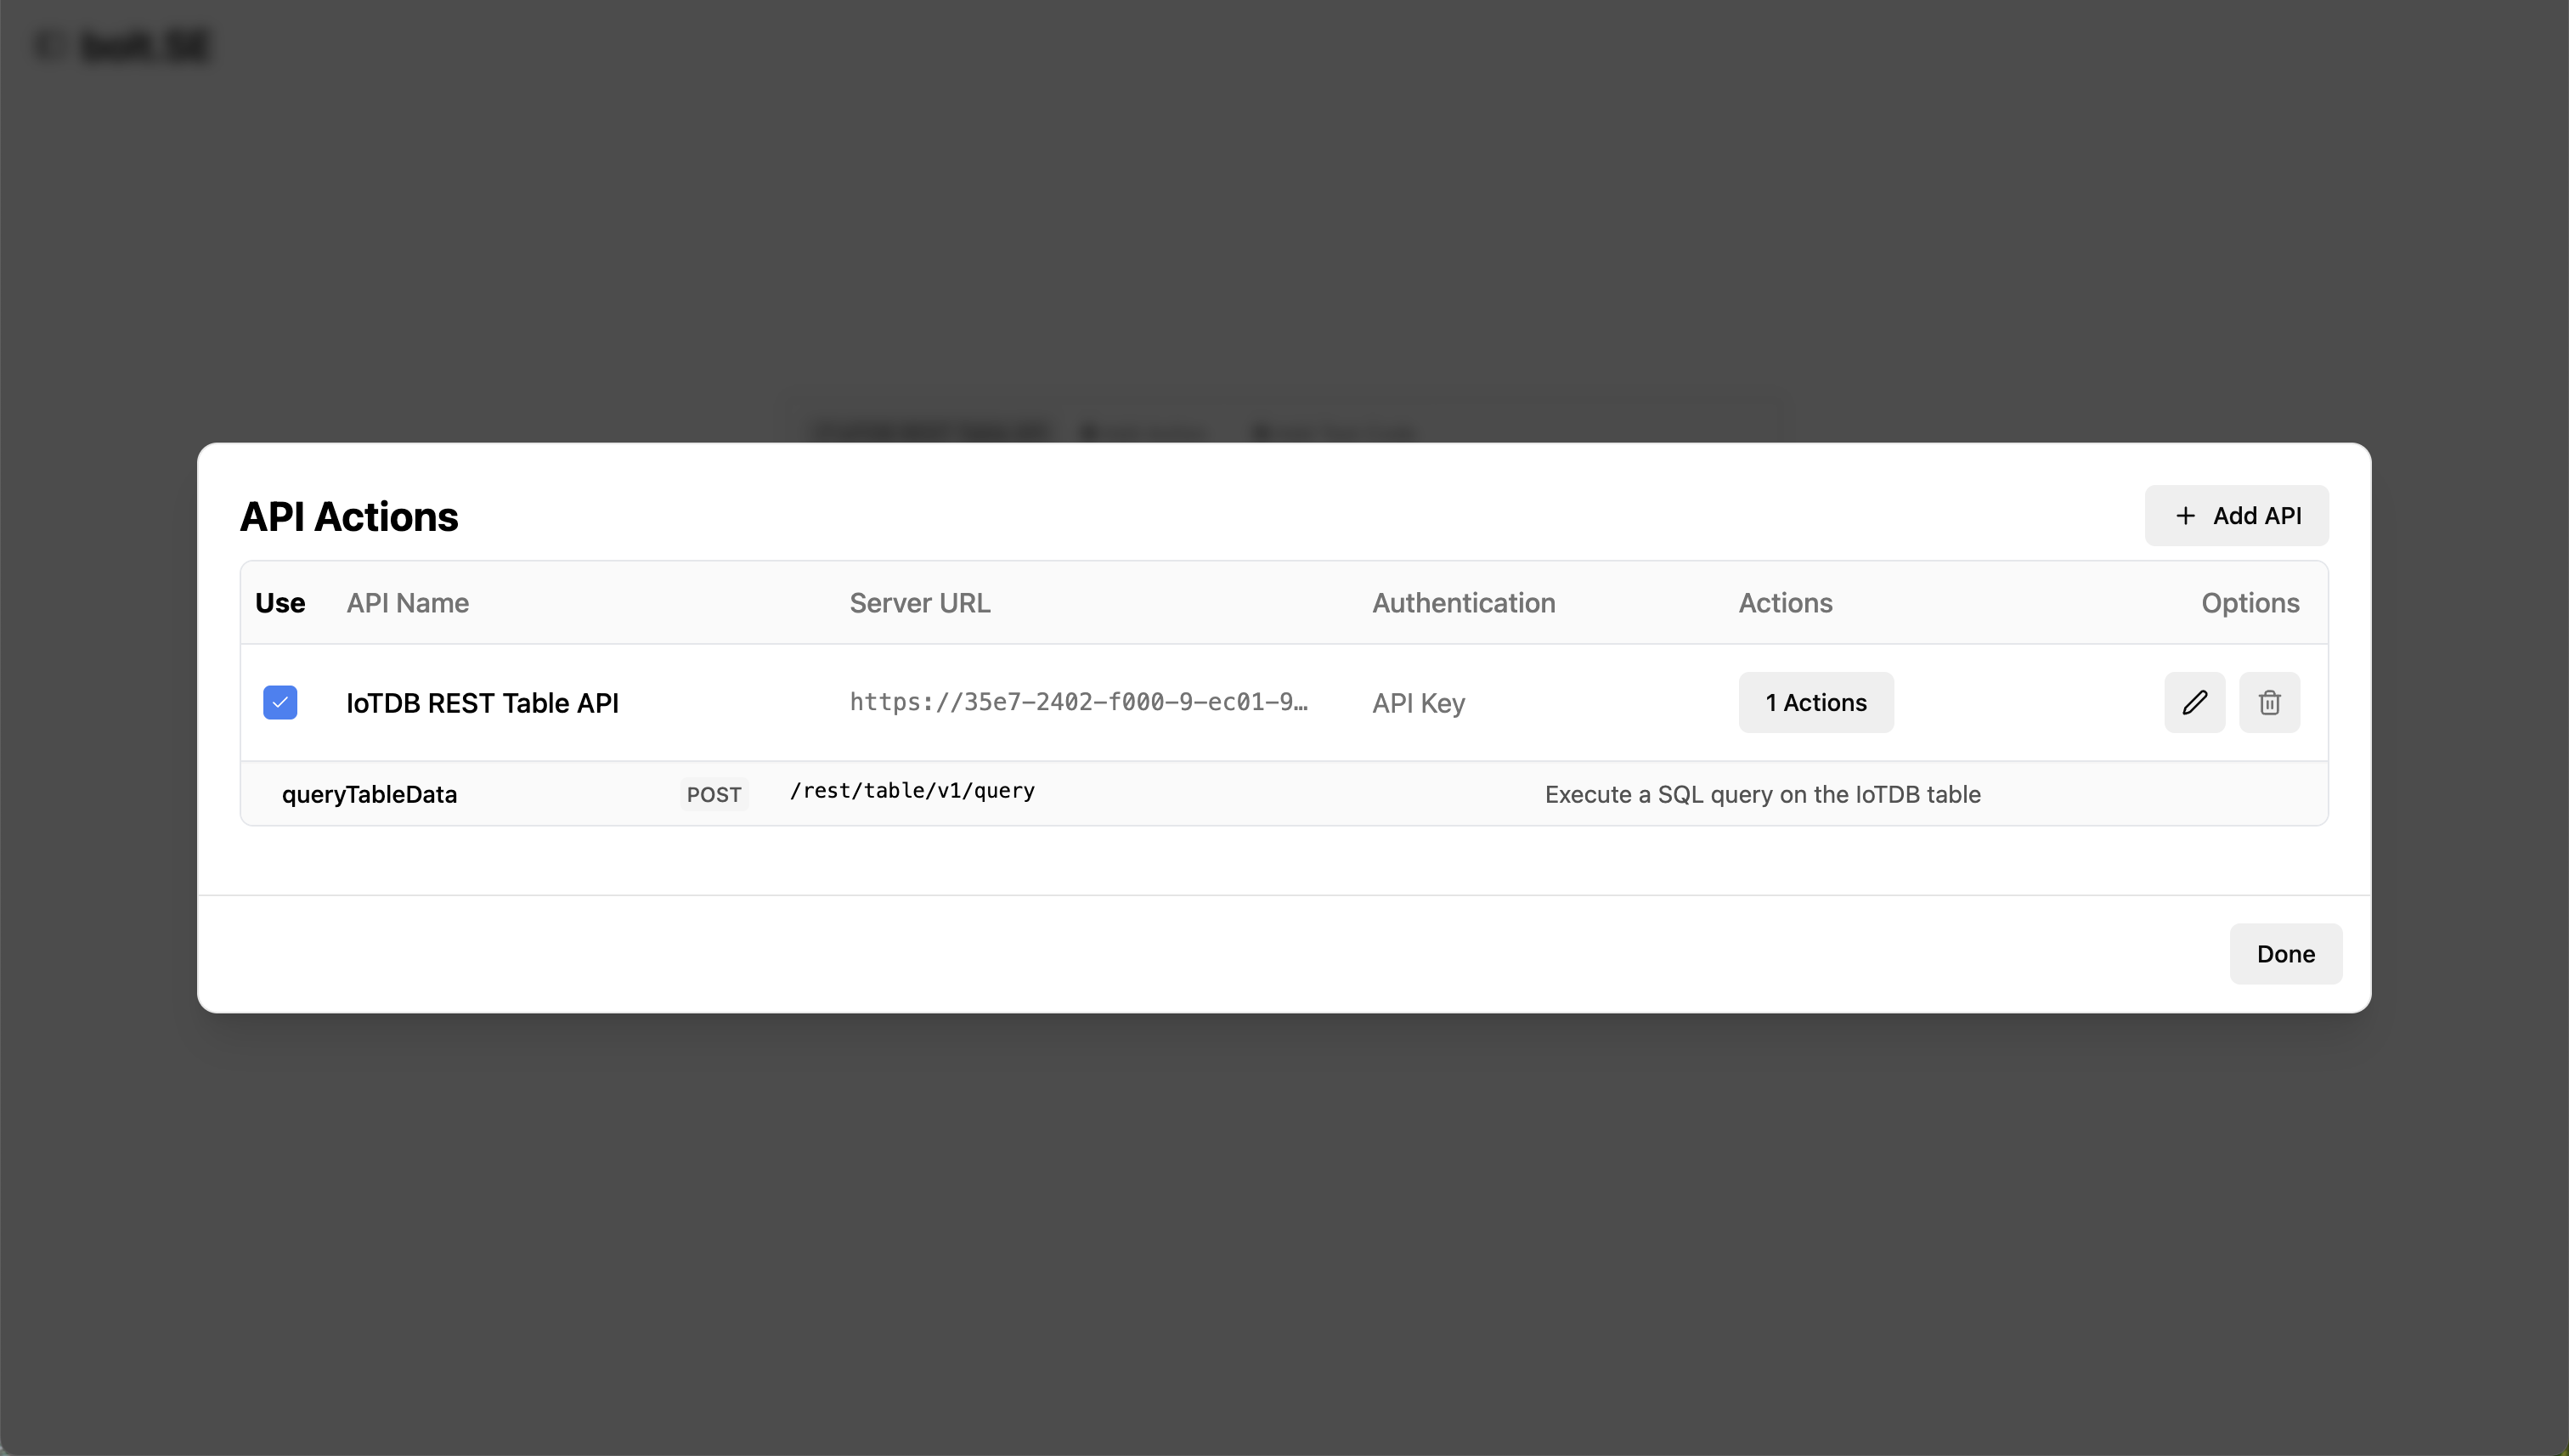
\includegraphics[width=.9\textwidth]{figures/screenshots/iotdb-demo/api-actions.png}
  \caption{动作列表仅包含 \textit{queryTableData},供 LLM 在提示中调用}
  \label{fig:api-actions}
\end{figure}

\subsection{一次自然语言提示的完整执行路径}

开发者随后输入提示:

\begin{quote}
\small
\textbf{Build a basic app that displays IoTDB data in a graph. Please use the tool to check the current database structure. Add a "Reload" button to refresh the data by calling the API.}
\end{quote}

LLM 先后调用三项 MCP 工具(图~\ref{fig:mcp-call}):

\begin{enumerate}
  \item \textit{list\_tables} $\rightarrow$ 确认仅有 \texttt{battery\_data};
  \item \textit{describe\_table} $\rightarrow$ 获取列名及类型;
  \item \textit{read\_query}(\verb|SELECT * FROM battery_data LIMIT 5|)$\rightarrow$ 抽样查看数值分布;
\end{enumerate}

随后调用 OpenAPI 动作 \textit{queryTableData}
生成完整查询逻辑与前端刷新函数。

\begin{figure}[htbp]
  \centering
  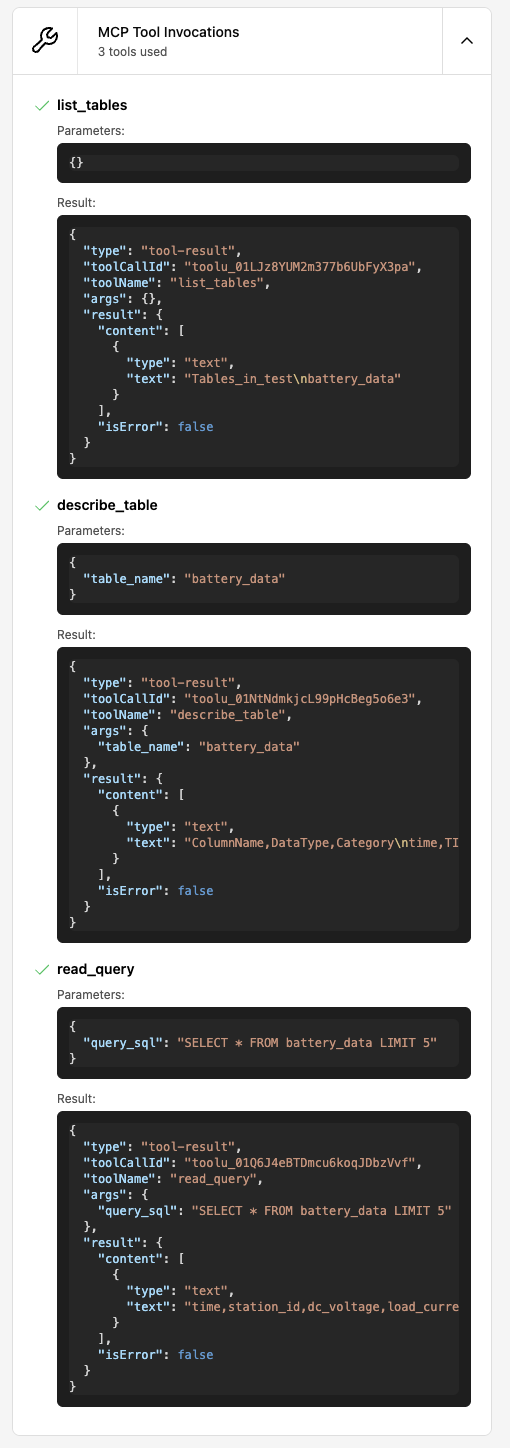
\includegraphics[width=.5\textwidth]{figures/screenshots/iotdb-demo/mcp-call.png}
  \caption{LLM 依次调用 \texttt{list\_tables}、\texttt{describe\_table}、\texttt{read\_query}}
  \label{fig:mcp-call}
\end{figure}

\subsection{自动生成并预览前端应用}

bolt.se 根据上述信息自动创建 Vite + React 工程(依赖安装、
文件骨架、\texttt{BatteryDataChart.jsx} 组件等),并运行在
内置 Workbench 容器中。  
图~\ref{fig:prompt-and-files} 显示 LLM 回复摘录与生成文件清单,
图~\ref{fig:app-preview} 则展示最终页面:折线图实时呈现
\texttt{DC Voltage}、\texttt{Load Current}、\texttt{Rectifier Current}
等曲线,顶部 \textit{Reload Data} 按钮触发
\texttt{queryTableData},下拉框可切换记录条数。

\begin{figure}[htbp]
  \centering
  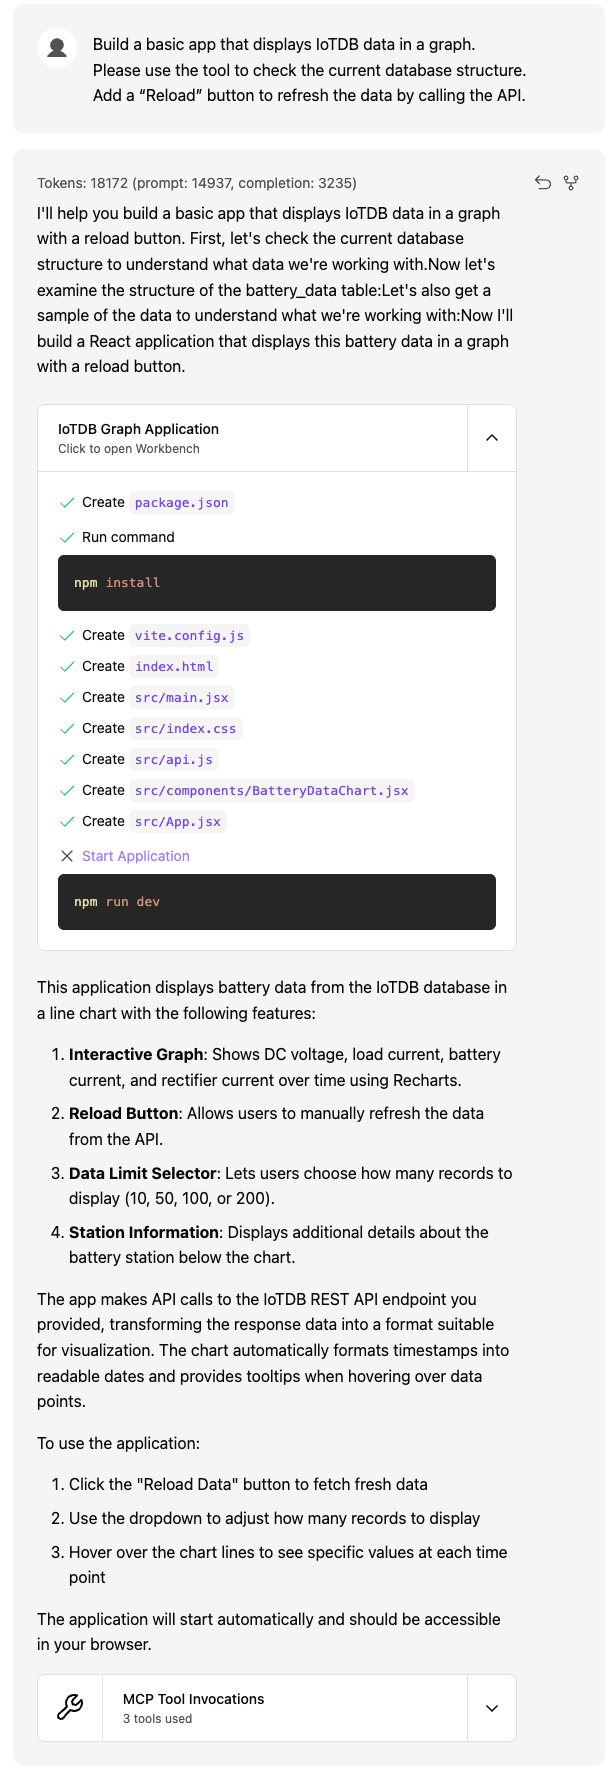
\includegraphics[width=.5\textwidth]{figures/screenshots/iotdb-demo/prompt-and-files.png}
  \caption{LLM 回复(左)与自动生成的文件任务列表(右)}
  \label{fig:prompt-and-files}
\end{figure}

\begin{figure}[htbp]
  \centering
  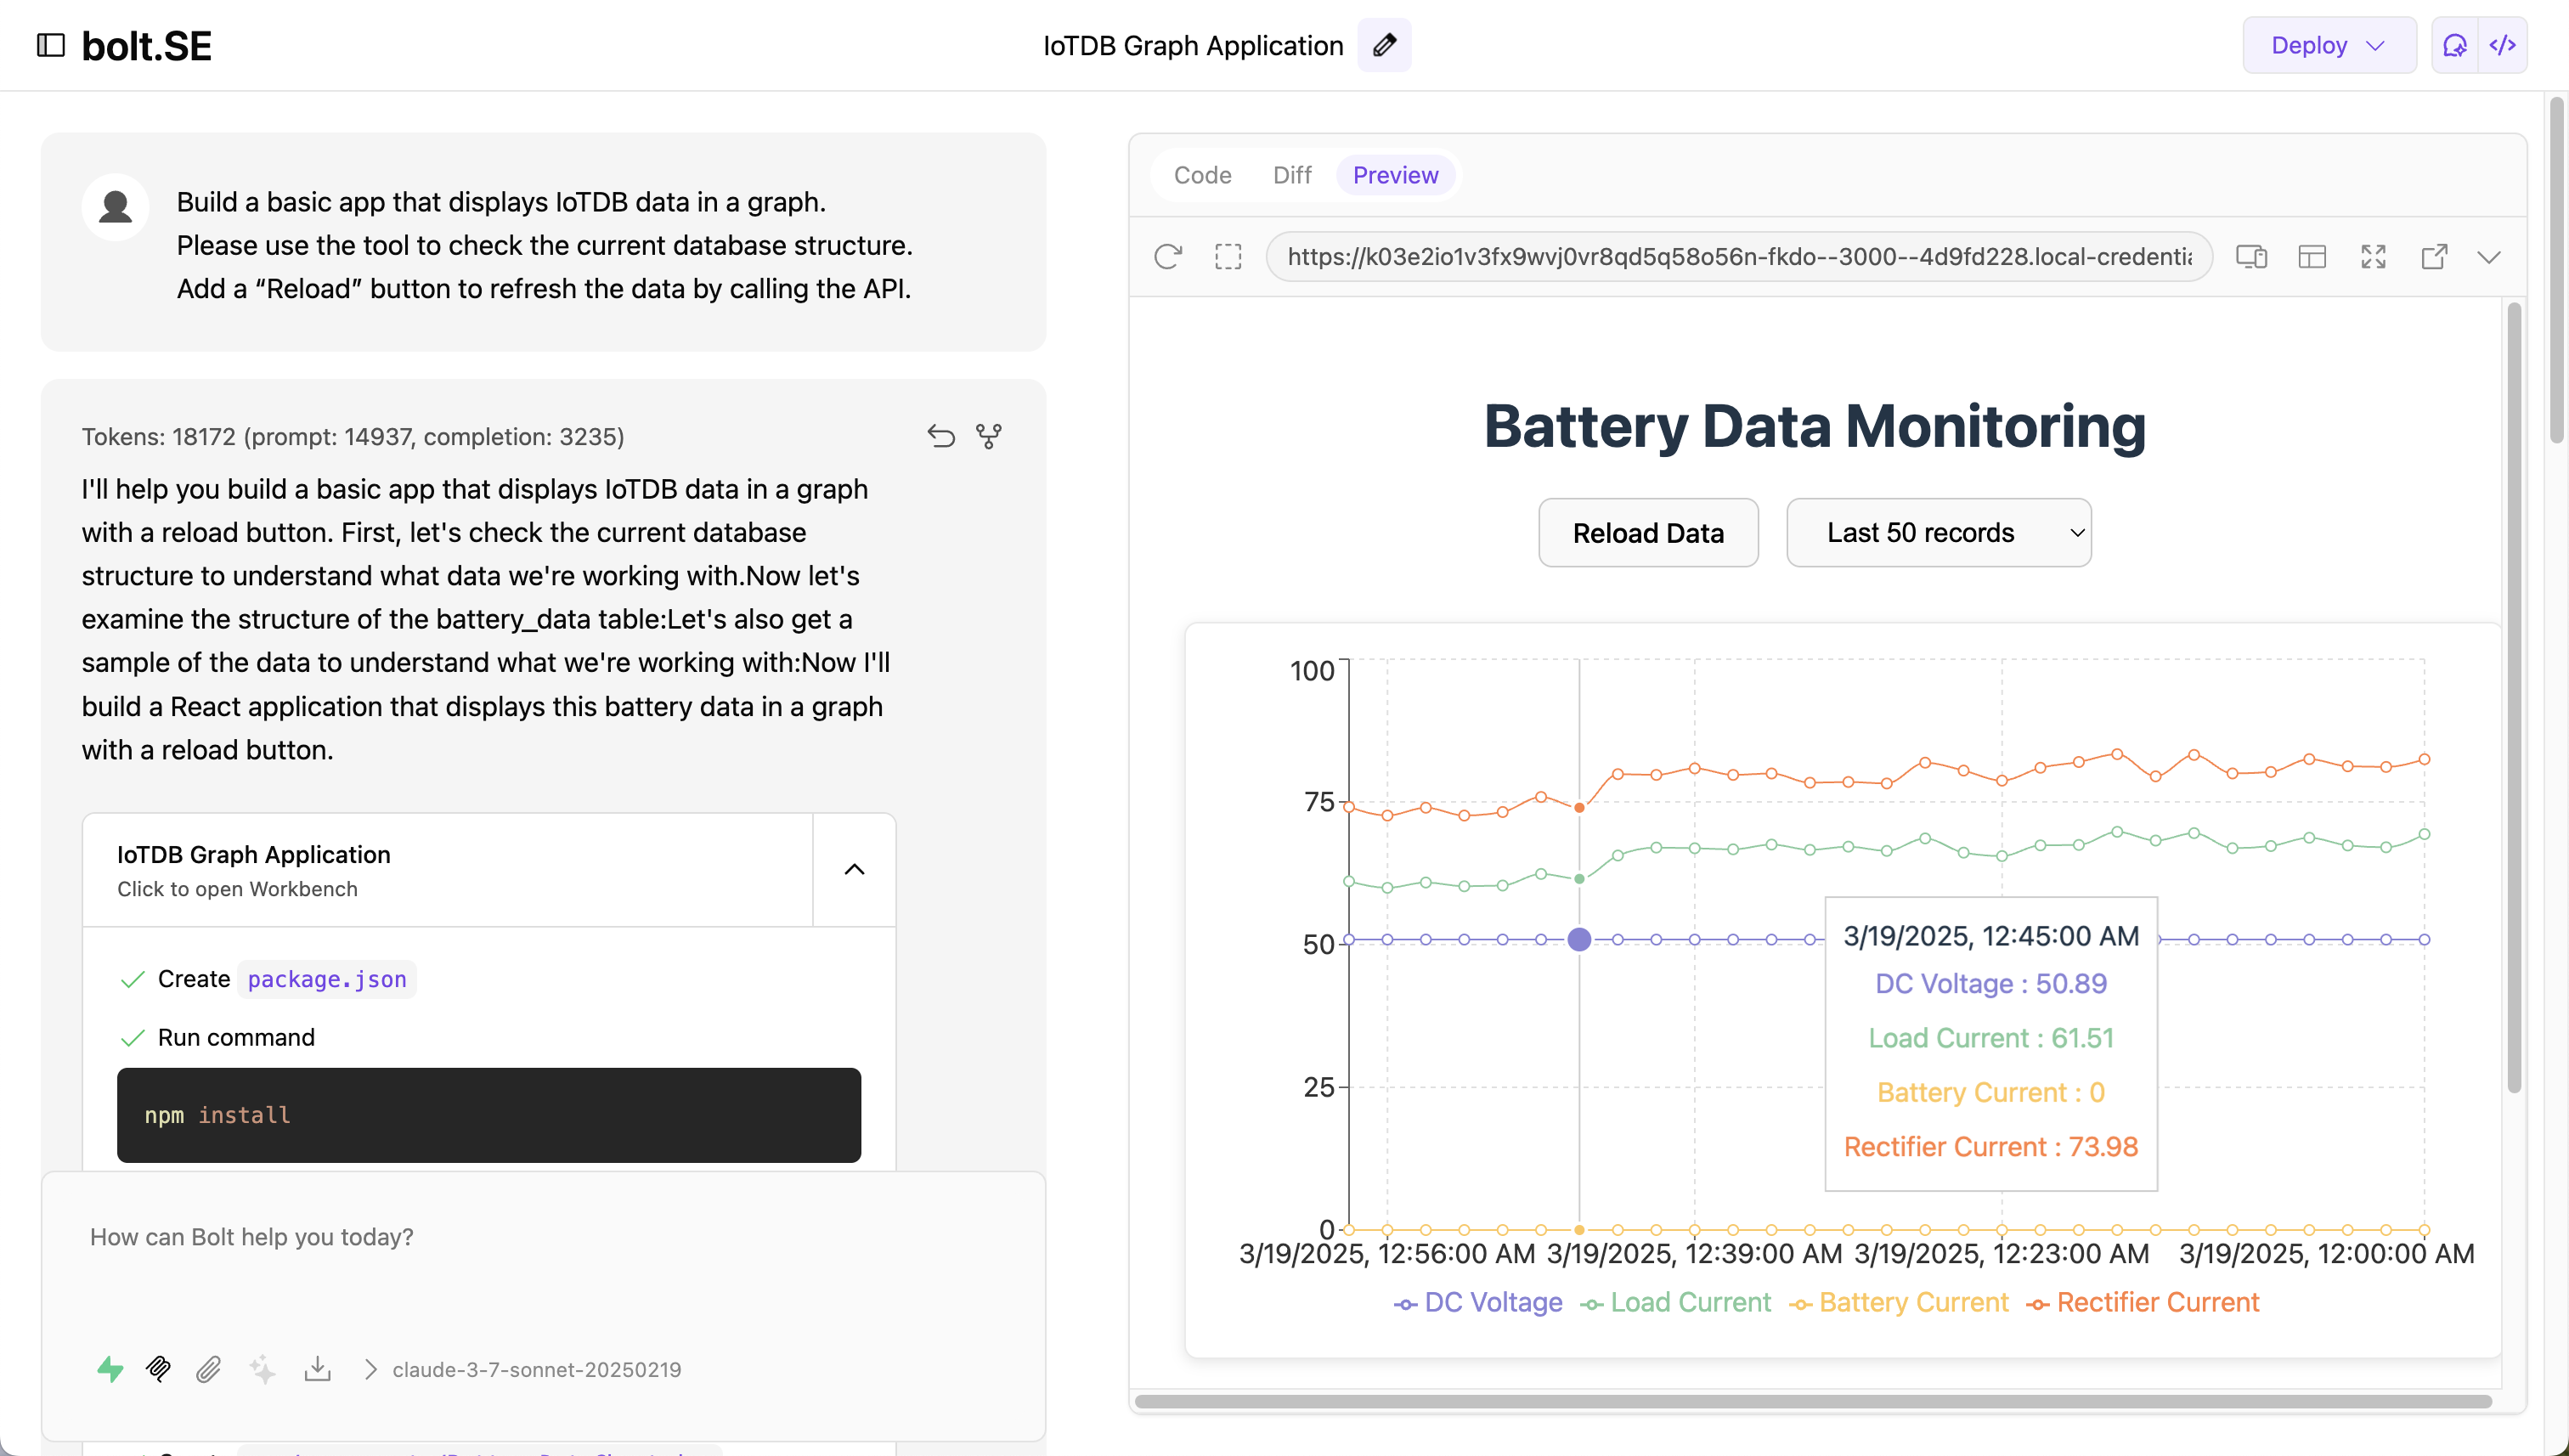
\includegraphics[width=.6\textwidth]{figures/screenshots/iotdb-demo/app-preview.png}
  \caption{Bolt.SE Workbench 预览:\textit{Battery Data Monitoring} 折线图与 \textit{Reload Data} 按钮}
  \label{fig:app-preview}
\end{figure}
